\solutionset

\begin{enumerate}

\item \textbf{The Bonnor-Ebert Sphere.}

\begin{enumerate}

\item For a uniform-density sphere with constant surface pressure, the terms that appear in the virial theorem are
\begin{eqnarray*}
\mathcal{W} & = & -\frac{3}{5} \frac{GM^2}{R} \\
\mathcal{T} & = & \frac{3}{2} M c_s^2 \\
\mathcal{T}_S & = & 4 \pi R^3 P_s.
\end{eqnarray*}
All other terms are zero. Virial equilibrium requires
\begin{eqnarray*}
0 & = & 2 (\mathcal{T} -\mathcal{T}_S) + \mathcal{W} \\
& = & 3 M c_s^2 - 8 \pi R^3 P_s - \frac{3}{5} \frac{G M^2}{R} \\
P_s & = & \frac{3 M c_s^2}{8\pi} \left[\frac{1}{R^3} - \left(\frac{G M}{5 c_s^2}\right)\frac{1}{R^4}\right].
\end{eqnarray*}
Notice that the first, positive, term in brackets dominates at large $R$, while the second, negative, one dominates at small $R$. Thus there must be a maximum at some intermediate value of $R$. To derive this maximum, we can take the derivative with respect to $R$. This gives
\begin{displaymath}
\frac{dP_s}{dR} = \frac{3 M c_s^2}{8\pi} \left[-\frac{3}{R^4} + \left(\frac{4 G M}{5 c_s^2}\right)\frac{1}{R^5}\right].
\end{displaymath}
Setting this equal to zero and solving, we find that the maximum occurs at
\begin{displaymath}
R = \frac{4 G M}{15 c_s^2}.
\end{displaymath}
Plugging this in for $P_s$, we obtain
\begin{displaymath}
P_s = \frac{10125}{2048\pi} \frac{c_s^8}{G^3 M^2} \approx 1.57 \frac{c_s^8}{G^3 M^2}.
\end{displaymath}

\item Since the gas is isothermal, we can substitute for $P$ to obtain
\begin{displaymath}
-c_s^2 \frac{1}{\rho} \frac{d}{dr}\rho = \frac{d}{dr}\phi
\end{displaymath}
The left-hand side can be re-written as
\begin{displaymath}
-c_s^2 \frac{d}{dr} \ln \rho = \frac{d}{dr}\phi,
\end{displaymath}
which makes the equation trivial to integrate:
\begin{displaymath}
-c_s^2 \ln \rho = \phi + \mathrm{const}.
\end{displaymath}
Fixing the constant of integration by the requirement that $\rho = \rho_c$ and $\phi=0$ at the origin, we have
\begin{displaymath}
\rho = \rho_c e^{-\phi/c_s^2}
\end{displaymath}

\item Substituting into the Poisson equation, we have
\begin{displaymath}
\frac{1}{r^2}\frac{d}{dr}\left(r^2 \frac{d\phi}{dr}\right) = 4 \pi G \rho_c e^{-\phi/c_s^2}
\end{displaymath}
Now define $\psi \equiv \phi/c_s^2$, giving
\begin{displaymath}
\frac{1}{r^2}\frac{d}{dr}\left(r^2 \frac{d\phi}{dr}\right) = \frac{4\pi G \rho_c}{c_s^2} e^{-\psi}.
\end{displaymath}
Finally, let
\begin{displaymath}
\xi \equiv \frac{r}{r_0},
\end{displaymath}
where 
\begin{displaymath}
r_0 = \frac{c_s}{\sqrt{4\pi G\rho_c}}.
\end{displaymath}
Substituting this in, we arrive at the desired equation:
\begin{displaymath}
\frac{1}{\xi^2}\frac{d}{d\xi}\left(\xi^2 \frac{d\psi}{d\xi}\right) = e^{-\psi}.
\end{displaymath}

\item For the purposes of numerical integration, it is most convenient to recast the problem as two first-order ODEs rather than a single second-order one. Let $\psi' = d\psi/d\xi$, and the system becomes
\begin{eqnarray*}
\frac{d\psi}{d\xi} & = & \psi' \\
\frac{d\psi'}{d\xi} & = & -2\frac{\psi'}{\xi} + e^{-\psi}.
\end{eqnarray*}
The only tricky part of the numerical solution to this system is the presence of a singularity in the equations at $\xi = 0$, which will cause numerical methods to choke. In this particular case it's not terrible to avoid this problem simply by starting the integration from a small but non-zero value of $\xi$ and setting $\psi = \psi' = 0$ at this point. However, this approach can run into problems for some equations, where the solution depends critically on the ratio of $\psi$ to $\psi'$ near the singular point. A better, more general method is to use a series expansion to solve the equation near the singularity, and then using that series expansion to numerically integrate starting from a small but non-zero value of $\xi$. Let $\psi = a_2 \xi^2 + a_3 \xi^3 + a_4 \xi^4 + \ldots$ in the vicinity of $\xi = 0$. Note that we know there is no constant or linear term due to the boundary conditions $\psi(0) = \psi'(0) = 0$. Substituting into the ODE and expanding, we obtain
\begin{displaymath}
6 a_2 + 12 a_3 \xi + O(\xi^2) = 1 + O(\xi^2).
\end{displaymath}
Since the equation must balance, we learn that $a_2 = 1/6$ and $a_3 = 0$, so the behavior of $\psi$ near $\xi = 0$ is $\psi = \xi^2/6 + O(\xi^4)$. Armed with this information, it is straightforward to integrate the equation numerically. Below is a simple Python code that can solve the problem:
\begin{verbatim}
import numpy as np
import matplotlib.pyplot as plt
from scipy.integrate import odeint

# definition of the derivatives
def derivs(y, x):
    return( [y[1], -2*y[1]/x+exp(-y[0])] )

# starting points
x0 = 1e-4
y0 = [x0**2/6, x0/3]

# solve the ode
x = np.linspace(x0, 8, 200)
ysol = odeint(derivs, y0, x)

# plot psi and exp(-psi) vs. x
plt.plot(x, ysol[:,0], lw=2, label=r'$\psi$')
plt.plot(x, np.exp(-ysol[:,0]), lw=2,
         label=r'$\rho/\rho_c$')
plt.legend(loc='upper left')
plt.xlabel(r'$\xi$')
\end{verbatim}
\begin{marginfigure}
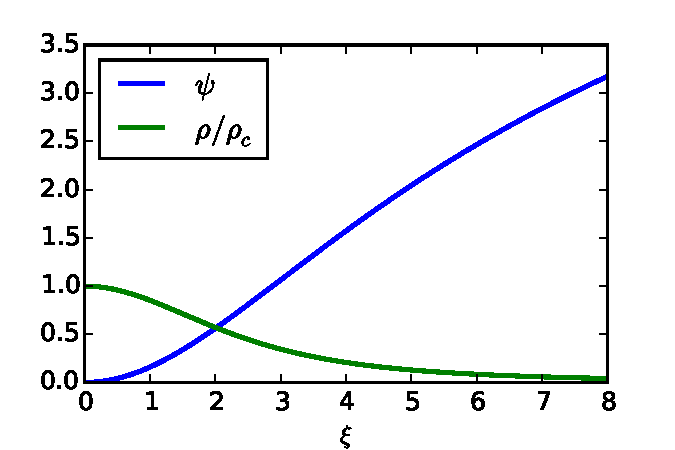
\includegraphics[width=\linewidth]{hw2sol1}
\caption[Solution to problem set~\thesolutionset, problem~\theenumi\theenumii]{
\label{fig:hw2sol1}
Dimensionless potential $\psi$ and density $\rho/\rho_c = e^{-\psi}$ found by solving the isothermal Lane-Emden equation.
}
\end{marginfigure}
The output produced by this code is shown in Figure \ref{fig:hw2sol1}.

\item As a first step, we can substitute in the dimensionless variables from the numerical solution:
\begin{displaymath}
M = 4\pi \int_0^R \rho r^2 \, dr = 4\pi r_0^3 \rho_c \int_0^{\xi_s} e^{-\psi} \xi^2 \, d\xi
\end{displaymath}
The integral can be evaluated by plugging using the isothermal Lane-Embden equation and then using the fundamental theorem of calculus:
\begin{displaymath}
\int_0^{\xi_s} e^{-\psi} \xi^2 \, d\xi = \int_0^{\xi_s} \frac{d}{d\xi}\left(\xi^2 \frac{d\psi}{d\xi}\right) \, d\xi
= \left(\xi^2 \frac{d\psi}{d\xi}\right)_{\xi_s}.
\end{displaymath}
Note that the term coming from the endpoint at $\xi=0$ vanishes because $\xi$ and $d\psi/d\xi$ are both $0$ there. The remainder of the problem is just a matter of substitution and manipulation:
\begin{eqnarray*}
M & = & 4\pi r_0^3 \rho_c \left(\xi^2 \frac{d\psi}{d\xi}\right)_{\xi_s} \\
& = & 4\pi \frac{c_s^3}{(4\pi G\rho_c)^{3/2}} \rho_c \left(\xi^2 \frac{d\psi}{d\xi}\right)_{\xi_s} \\
& = & \frac{c_s^4}{\sqrt{4\pi G^3 \rho_c P_s/\rho_s}} \left(\xi^2 \frac{d\psi}{d\xi}\right)_{\xi_s} \\
& = & \frac{c_s^4}{\sqrt{4\pi G^3 P_s}}  \left(e^{-\psi/2}\xi^2 \frac{d\psi}{d\xi}\right)_{\xi_s}.
\end{eqnarray*}

\item Using the numerical results from above, and recalling that $\rho_c/\rho = e^{\psi}$, this is a fairly simple addition to the program. To get a bit more range on the density contrast, it is helpful to extend the range of $\xi$ a bit further than for the previous problem. A simple solution, to be executed after the previous code, is
\begin{verbatim}
# solve the ode on a slightly larger grid
x = np.linspace(x0, 1e3, 500000)
ysol = odeint(derivs, y0, x)

# Get density constrast and m
contrast = np.exp(ysol[:,0])
m = (x**2 * np.exp(-ysol[:,0]/2) * ysol[:,1]) \
    / np.sqrt(4.0*np.pi)

# Plot
plt.clf()
plt.plot(contrast, m, lw=2)
plt.xscale('log')
plt.xlabel(r'$\rho_c/\rho_s$')
plt.ylabel('m')
plt.xlim([1,1e4])
\end{verbatim}
\begin{marginfigure}
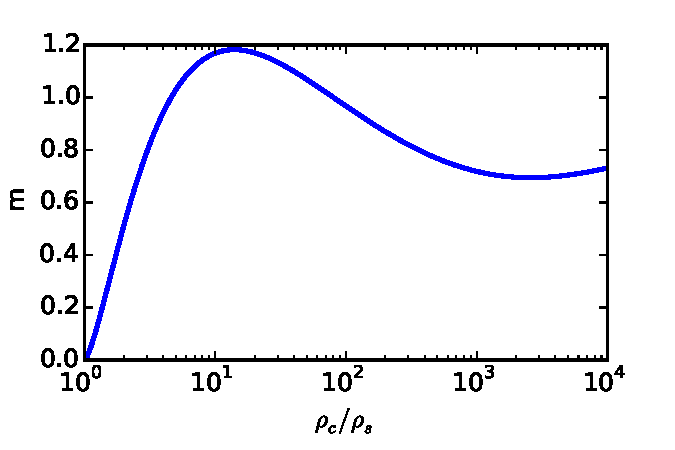
\includegraphics[width=\linewidth]{hw2sol2}
\caption[Solution to problem set~\thesolutionset, problem~\theenumi\theenumii]{
\label{fig:hw2sol2}
Dimensionless mass $m$ versus dimensionless density contrast $\rho_c/\rho_s$ found by solving the isothermal Lane-Emden equation.
}
\end{marginfigure}
The output produced by this code is shown in Figure \ref{fig:hw2sol2}. The maximum value of $m$ (obtained via \verb=np.amax(m)=) is 1.18. The maximum is at (found via \verb=contrast[np.argmax(m)-1]=) $\rho_c/\rho_s = 14.0$.

\item The dimensionless and dimensional mass are related by
\begin{displaymath}
m = \frac{P_s^{1/2} G^{3/2} M}{c_s^4},
\end{displaymath}
so the maximum surface pressure is
\begin{displaymath}
P_{s,\rm max} = m_{\rm max}^2 \frac{c_s^8}{G^3 M^2},
\end{displaymath}
where $m_{\rm max}$ is the maximum value of $m$ produced by the numerical solution in the previous part. Plugging this in, we have
\begin{displaymath}
P_{s,\rm max} \approx 1.40 \frac{c_s^8}{G^3 M^2},
\end{displaymath}
which is only slightly different than the result we got for the uniform sphere value in part (a) -- a coefficient of 1.40 instead of 1.57.

\item The maximum mass is
\begin{displaymath}
M_{\rm BE} = m_{\rm max} \frac{c_s^4}{P_s^{1/2} G^{3/2}} \approx 1.18  \frac{c_s^4}{P_s^{1/2} G^{3/2}}
\end{displaymath}
At $T = 10$ K, a gas with $\mu=3.9\times 10^{-24}$ g has a sound speed $c_s = 0.19$ km s$^{-1}$. Plugging this in, together with the given value of $P_s$, we find $M_{\rm BE} = 0.67$ $\msun$.

\end{enumerate}

\item \textbf{Driving Turbulence with Protostellar Outflows.}

\begin{enumerate}

\item The escape speed at the stellar surface, and thus the launch velocity of the wind, is $v_w = \sqrt{2G M_*(t)/R_*}$, where $M_*(t)$ is the star's instantaneous mass. The momentum flux associated with the wind is therefore $\dot{p}_w = f \dot{M}_d v_w$. The accretion rate onto the star is $\dot{M}_* = (1-f) \dot{M}_d$. Thus at a time $t$ after the star has started accreting, we have $M_*(t) = (1-f) \dot{M}_d t$, and
\begin{displaymath}
\dot{p}_w = f (1-f)^{1/2} \dot{M}_d^{3/2} \left(\frac{2G}{R_*}\right)^{1/2} t^{1/2}.
\end{displaymath}
The time required to accrete up to the star's final mass is $t_f = M_*/\dot{M}_* = (1-f)^{-1} M_*/\dot{M}_d$, where $M_*$ is the final mass. To obtain the wind momentum per unit stellar mass, we must integrate $\dot{p}_w$ over the full time it takes to build up the star, then divide by the star's mass. Thus we have
\begin{eqnarray*}
\langle p_w\rangle & = & \frac{1}{M_*} \int_0^{(1-f)^{-1} M_*/\dot{M}_d} f (1-f)^{1/2} \dot{M}_d^{3/2} \left(\frac{2G}{R_*}\right)^{1/2} t^{1/2}\, dt \\
& = & \frac{2}{3} \frac{f}{1-f} \sqrt{\frac{2 G M_*}{R_*}}.
\end{eqnarray*}
Evaluating numerically for the given values of $f$, $M_*$, and $R_*$ gives $\langle p_w\rangle = 19$ km s$^{-1}$ $\msun^{-1}$.

\item Each outflow carries momentum $\langle p_w\rangle M_*$, and thus when it decelerates to terminal velocity $\sigma$ the mass it has swept-up must be $M_w = (\langle p_w\rangle/\sigma) M_*$. The associated kinetic energy of a single outflow is 
\begin{displaymath}
\mathcal{T}_w = \frac{1}{2} M_w \sigma^2 = \frac{1}{2} M_* \langle p_w\rangle \sigma.
\end{displaymath}
If the total star formation rate is $\dot{M}_{\rm cluster}$, then the rate at which new stars form is $\dot{M}_{\rm cluster}/M_*$. The rate of kinetic energy injection is therefore
\begin{eqnarray*}
\dot{\mathcal{T}} & = & \frac{\dot{M}_{\rm cluster}}{M_*} \mathcal{T}_w \\
& = & \frac{1}{2} \dot{M}_{\rm cluster} \langle p_w\rangle \sigma \\
& = & \frac{1}{3}\left(\frac{f}{1-f}\right) \dot{M}_{\rm cluster} \sigma \sqrt{\frac{2 G M_*}{R_*}}.
\end{eqnarray*}

\item The decay time is $L/\sigma$, to the decay rate must be the cloud kinetic energy $(3/2) M \sigma^2$ divided by this time. Thus
\begin{displaymath}
\dot{\mathcal{T}}_{\rm dec} = -\frac{3}{2} \frac{M \sigma^3}{L}.
\end{displaymath}
If we now set $\dot{\mathcal{T}}_w = -\dot{\mathcal{T}}_{\rm dec}$, we can solve for $\dot{M}_{\rm cluster}$. Doing so gives
\begin{displaymath}
\dot{M}_{\rm cluster} = \frac{9}{2}\left(\frac{1-f}{f}\right) \sqrt{\frac{R_*}{2 G M_*}} \frac{\sigma^2}{L} M.
\end{displaymath}
Using the Larson relations to evaluate this, note that $\sigma^2/L = \sigma_1^2/\mbox{pc} \equiv a_c = 3.2\times 10^{-9}$ cm s$^{-1}$ is constant, and we are left with
\begin{displaymath}
\dot{M}_{\rm cluster} = \frac{9}{2}\left(\frac{1-f}{f}\right) \sqrt{\frac{R_*}{2 G M_*}} a_c M_1 \left(\frac{L}{\mbox{pc}}\right)^2.
\end{displaymath}
Evaluating numerically for the given values of $L$ produces the results below:
\begin{center}
\begin{tabular}{l|ccc}
& $L=1$ pc & $L = 10$ pc & $L = 100$ pc \\ \hline
$\dot{M}_{\rm cluster}$ [$\msun$ yr$^{-1}$] & $1.6\times 10^{-5}$ & $1.6\times 10^{-3}$ & $1.6\times 10^{-1}$
\end{tabular}
\end{center}

\item The mass converted into stars in 1 free-fall time is $\dot{M}_{\rm cluster} t_{\rm ff}$, so the quantity we want to compute is
\begin{displaymath}
f = \frac{\dot{M}_{\rm cluster}}{M} t_{\rm ff} \equiv \frac{t_{\rm ff}}{t_*},
\end{displaymath}
where $t_*$ is the star formation timescale. From the previous part, we have
\begin{displaymath}
t_*^{-1} = \frac{\dot{M}_{\rm cluster}}{M} =  \frac{9}{2}\left(\frac{1-f}{f}\right) \sqrt{\frac{R_*}{2 G M_*}} a_c = 0.16\mbox{ Myr}^{-1}.
\end{displaymath}
The free-fall time is
\begin{eqnarray*}
t_{\rm ff} & = & \sqrt{\frac{3\pi}{32 G \rho}} = \sqrt{\frac{3\pi L^3}{32 G M}} = \sqrt{\frac{3\pi L_1^3}{32 G M_1}} \left(\frac{L}{L_1}\right)^{1/2} \\
& = & 0.81 \left(\frac{L}{L_1}\right)^{1/2}\mbox{ Myr},
\end{eqnarray*}
where $L_1 = 1$ pc. Thus we have
\begin{displaymath}
f = \frac{t_{\rm ff}}{t_*} = 0.13 \left(\frac{L}{L_1}\right)^{1/2}.
\end{displaymath}
Evaluating for $L = 1$, $10$, and $100$ pc, we get $f = 0.13$, $0.42$, and $1.3$, respectively. We therefore conclude that protostellar outflows may be a significant factor in the driving the turbulence on $\sim 1$ pc scales, and cannot be ignored there. However, they become increasingly less effective at larger size scales, and can probably be neglected at the scales of entire GMCs, $\sim 10-100$ pc.

\end{enumerate}

\item \textbf{Magnetic Support of Clouds.}

\begin{enumerate}

\item The virial ratio is (omitting constant factors of order unity)
\begin{displaymath}
\alpha_{\rm vir}\sim \frac{\sigma^2 R}{G M}.
\end{displaymath}
The Alfv\'en Mach number is the ratio of the velocity dispersion to the Alfv\'en speed
\begin{displaymath}
v_A \sim \frac{B}{\sqrt{\rho}} \sim \frac{B R^{3/2}}{M^{1/2}}.
\end{displaymath}
Thus
\begin{displaymath}
\mathcal{M}_A \sim \frac{\sigma M^{1/2}}{B R^{3/2}}.
\end{displaymath}
To rewrite this in terms of $M_\Phi$, we can eliminate $B$ from this expression by writing
\begin{displaymath}
B \sim \frac{M_\Phi G^{1/2}}{R^2},
\end{displaymath}
giving
\begin{displaymath}
\mathcal{M}_A \sim \frac{\sigma}{M_\Phi} \sqrt{\frac{MR}{G}}
\end{displaymath}
Similarly, we can eliminate $\sigma$ using the definition of the virial ratio:
\begin{displaymath}
\sigma \sim \sqrt{\alpha_{\rm vir}\frac{G M}{R}},
\end{displaymath}
and substituting this in gives
\begin{displaymath}
\mathcal{M}_A \sim \alpha_{\rm vir}^{1/2} \mu_\Phi.
\end{displaymath}

\item The expression derived in part (a) does indeed show that, if any of two of the three quantities $\mathcal{M}_A$, $\alpha_{\rm vir}$, and $\mu_\Phi$ are of order unity, the third one must be as well. Intuitively, this is because the various quantities are measures of energy ratios. Roughly speaking, $\mathcal{M}_A^2$ measures the ratio of kinetic (including thermal) energy to magnetic energy; $\alpha_{\rm vir}$ measures the ratio of kinetic to gravitational energy; and $\mu_\Phi^2$ represents the ratio of gravitational to magnetic energy. If any two of these are of order unity, then this implies that gravitational, kinetic, and magnetic energies are all of the same order. However, this in turn implies that the third dimensionless ratio should also be of order unity as well. For example, if $\mathcal{M}_A \sim \alpha_{\rm vir} \sim 1$, then this implies that kinetic energy is comparable to magnetic energy, and kinetic energy is also comparable to gravitational energy. In turn, this means that gravitational and mantic energy are comparable, in which case $\mu_\Phi \sim 1$.

\item If we have a cloud that is supported, it must have $\alpha_{\rm vir}\sim 1$. However, if the cloud is turbulent then it will naturally also go to $\mathcal{M}_A \sim 1$. This means that we are likely to measure $\mu_{\Phi}\sim 1$ even if the cloud is magnetically supercritical and not supported by its magnetic field. We would only ever expect to get $\mu_{\Phi} \gg 1$, indicating a lack of magnetic support, if the cloud were either non-virialized ($\alpha_{\rm vir} \gg 1$ or $\ll 1$) or non-turbulent.

\end{enumerate}


\end{enumerate}


